\documentclass[xcolor=dvipsnames]{beamer}
\usepackage{ucs}
\usepackage[T1]{fontenc}
\usepackage[utf8x]{inputenc}
\usepackage{overpic}
\usepackage{lmodern}
\usepackage[defaultsans]{droidsans}

\usepackage{subfigure}

\renewcommand*\familydefault{\sfdefault} %% Only if the base font of the document is to be typewriter style

% Set colors to uni-colors
\setbeamercolor{frametitle}{fg=NavyBlue}
\setbeamercolor{normal text}{bg=white,fg=black!95}
\setbeamercolor{section in toc}{fg=NavyBlue}
\setbeamercolor{title}{fg=NavyBlue}
\setbeamercolor{titlelike}{fg=NavyBlue}
\setbeamercolor{itemize item}{fg=NavyBlue}
\setbeamercolor{caption name}{fg=NavyBlue}
\setbeamercolor{section in head/foot}{fg=NavyBlue}
\setbeamercolor{subsection in head/foot}{fg=NavyBlue}
\setbeamercolor{bibliography entry author}{fg=NavyBlue}

\title{Final presentation master lab}
\subtitle{A visual artifact detector for ITS.APE}
\author{Felix Rossmann} 
\date{2nd of April 2019}

\setbeamertemplate{navigation symbols}{}

\setbeamertemplate{footline}[text line]{%
	\begin{minipage}[b]{108mm}
		\insertauthor \hfill \inserttitle\hspace{1mm}- \hspace{1mm}\insertframenumber{} / \inserttotalframenumber\hspace*{2ex} \hfill {
\includegraphics[scale=0.1]{unilogo.pdf}}
		%
		%neue Navigationsleiste
	\end{minipage}
}

\setbeamertemplate{headline}{%
	\begin{beamercolorbox}{section in head/foot}
		\vskip2pt\insertnavigation{\paperwidth}\vskip2pt
	\end{beamercolorbox}%
}

\setbeamerfont{frametitle}{series=\bfseries,size={\fontsize{16}{18}}}

\begin{document}
	\begin{frame}
		\titlepage
	\end{frame}
	
	\begin{frame}
		\frametitle{Structure}
		\tableofcontents
	\end{frame}
	
	\section{Introduction} 
	\begin{frame}
		\frametitle{What's ITS.APE and why does it need a detector?}
		% Intro chapter
		ITS.APE: IT-Security Awareness Penetration Testing Environment
		
		\begin{itemize}
			\item Framework for human pentesting \cite{itsape}
			\pause
			\item Deploys \emph{artifacts} of a \emph{type} based on \emph{recipes}
			\item Measures the response to those artifacts
		\end{itemize}
		\pause
		\vspace*{1cm}~\\
		When to start measuring? $\Rightarrow$ Visibility in user's desktop
	\end{frame}
	
	\begin{frame}
		\frametitle{Artifact's visual cues -- examples}
		% Examples of artifacts
		\begin{figure}[h!]
			\subfigure{
				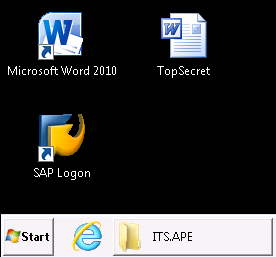
\includegraphics[width=0.3\textwidth]{fig/artifact-ex3}
				}\qquad
			\subfigure{
				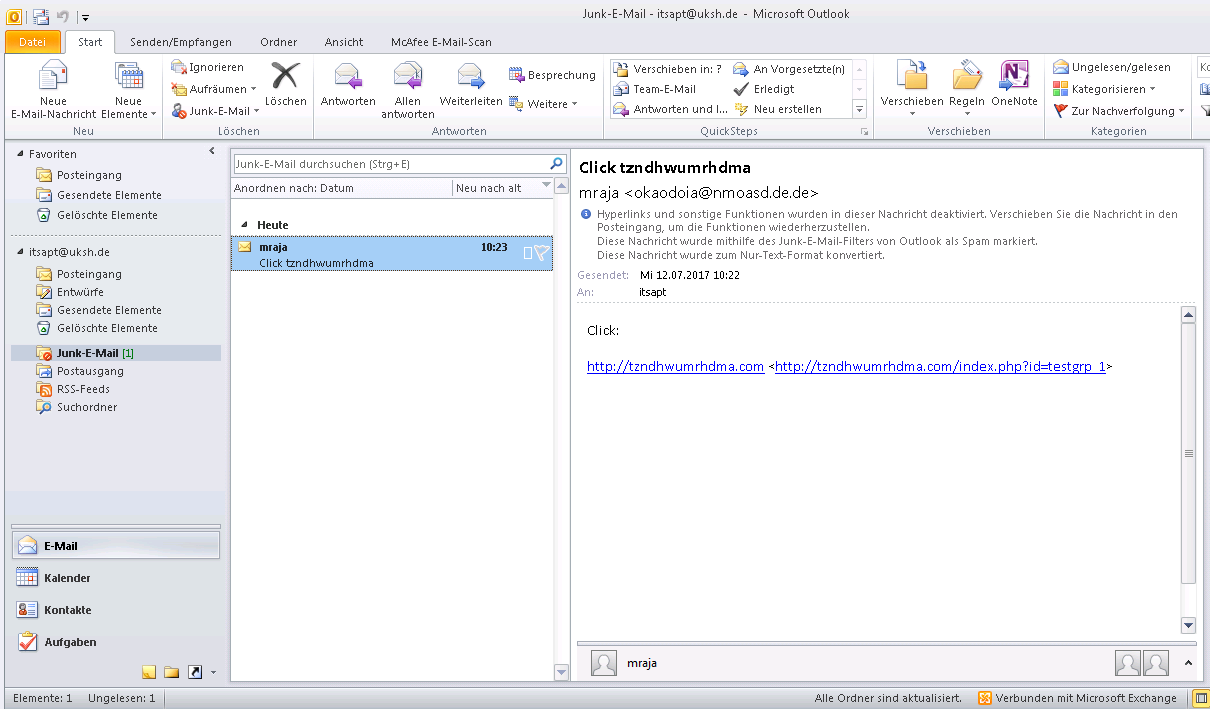
\includegraphics[width=0.55\textwidth]{fig/artifact-ex1}
				}\\
			\subfigure{
				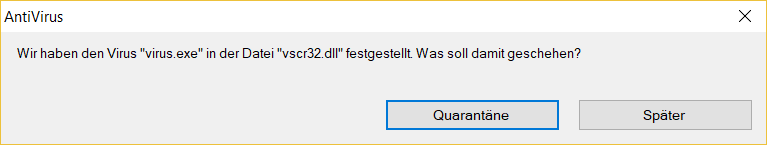
\includegraphics[width=0.55\textwidth]{fig/artifact-ex2}
				}\qquad
			\subfigure{
				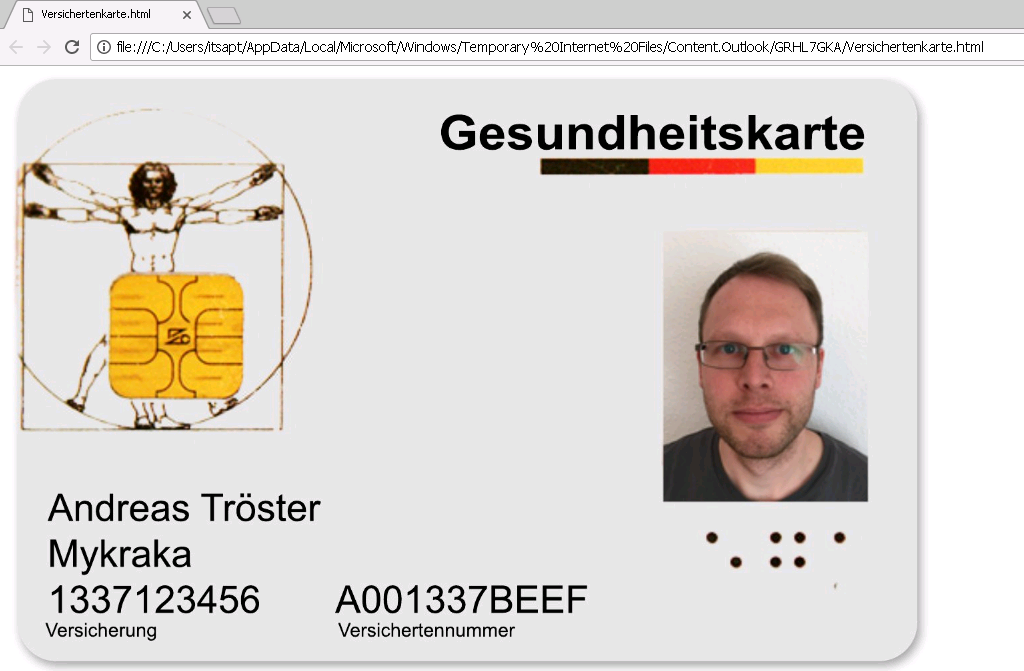
\includegraphics[width=0.3\textwidth]{fig/artifact-ex4}
				}\\
			\caption{Examples for artifacts' reference images}\label{fig:artifact-examples}
		\end{figure}
	\end{frame}
	
	\begin{frame}
		\frametitle{A new tool: The VAD}
		% Measures
		VAD: Visual artifact detector\\
		Measures of quality:
		\begin{enumerate}
			\item High rate of successful detection (\emph{sensitivity}, \emph{detection rate})
			\item Low resource consumption (esp. runtime)
		\end{enumerate}
		\pause
		\vspace*{1cm}~\\
		Target environment: Low-tier office hardware (Windows 7)\\
		$\Rightarrow$ Runtime of at most several seconds\\
		$\Rightarrow$ No CUDA, Windows 7 32 bit console application
	\end{frame}
	
	\section{Methods}
	\begin{frame}
		\frametitle{Software design}
		% Requirements
		\begin{itemize}
			\item Separate tool from ITS.APE client service
			\item Same machine as client: User's privacy
		\end{itemize}
	\end{frame}
	
	\subsection{Design decisions}
	\begin{frame}
		\frametitle{Major design decisions}
		% Used libraries
		\begin{itemize}
			\item Image recognition library $\Rightarrow$ OpenCV \cite{opencv}
			\item Wrapper Emgu CV (3.4.3) to use in C\# \cite{emgucv}
			\item .NET Framework (4.7.2) \cite{dotnet4_7_2}
			\item Installer setup
		\end{itemize}
	\end{frame}
	
	\subsection{Technical overview}
	\begin{frame}
		\frametitle{How is it implemented?}
		% Pic: Example run
		\begin{figure}[h]
			\centering
			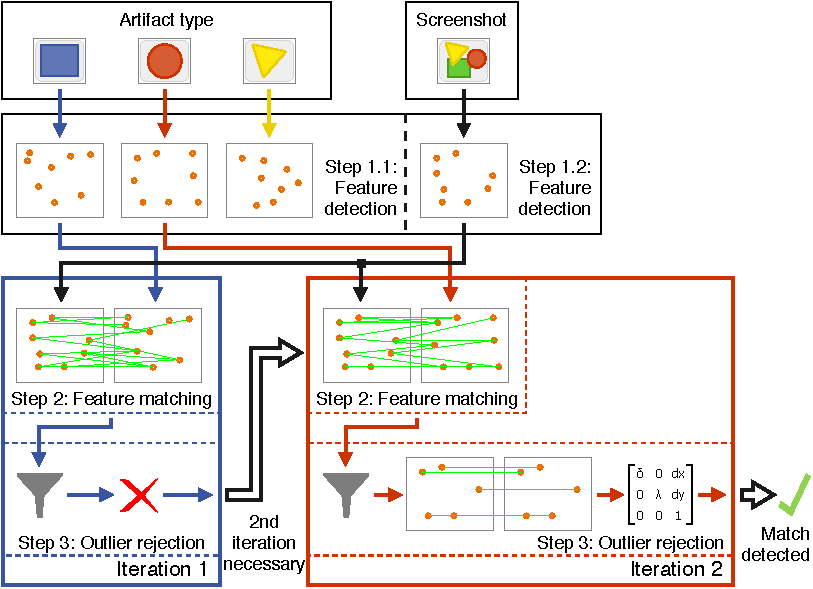
\includegraphics[width=0.8\textwidth]{fig/rec-process}
			\caption{Exemplary recognition process diagram.}\label{fig:recognition-process}
		\end{figure}
	\end{frame}
	
	\section{Evaluation}
	\begin{frame}
		\frametitle{Evaluation of the implementation}
		% Techniques
		\begin{itemize}
			\item Virtual machine, Oracle's VirtualBox \cite{virtualbox}
			\item Virtual CPU with 1.4 GHz
			\item 2GB of RAM
			\item Windows 7 without any other software
		\end{itemize}
		\vspace*{1cm}~\\
		\pause
		% Setup 1
		First setup for evaluation:
		\begin{itemize}
			\item 25 artifact types from recipes repository (A 1 to A 25)
			\item 365 screenshots generated (see next slide)
			\item 9125 executions of the VAD
		\end{itemize}
	\end{frame}
	
	\begin{frame}
		% Examples for setup 1
		\begin{figure}[h!]
			\subfigure{
				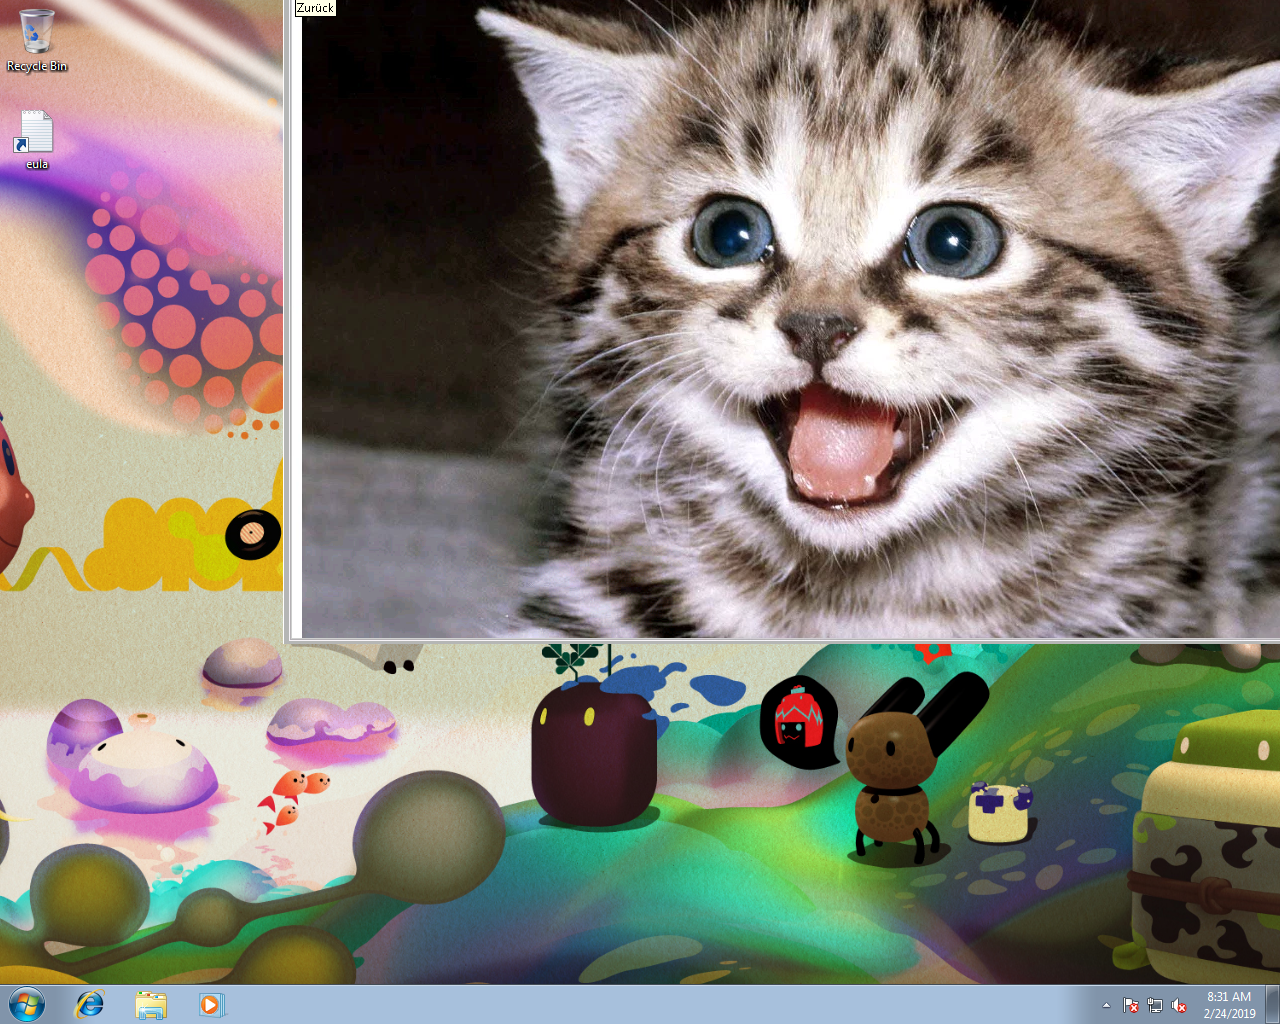
\includegraphics[width=0.4\textwidth]{fig/setup1-ex1}
				}\qquad
			\subfigure{
				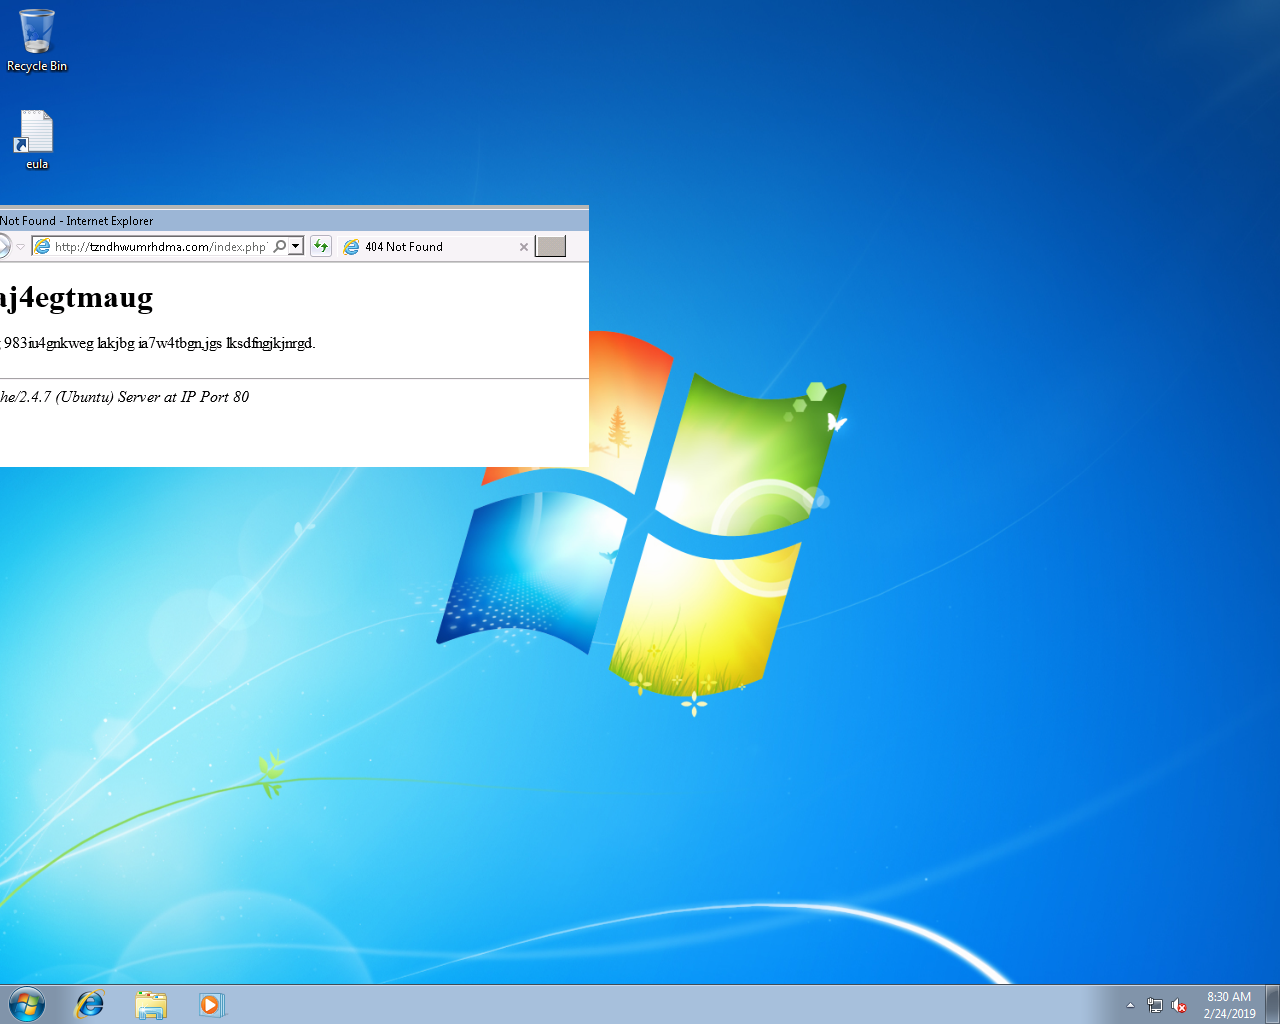
\includegraphics[width=0.4\textwidth]{fig/setup1-ex2}
				}\\
			\subfigure{
				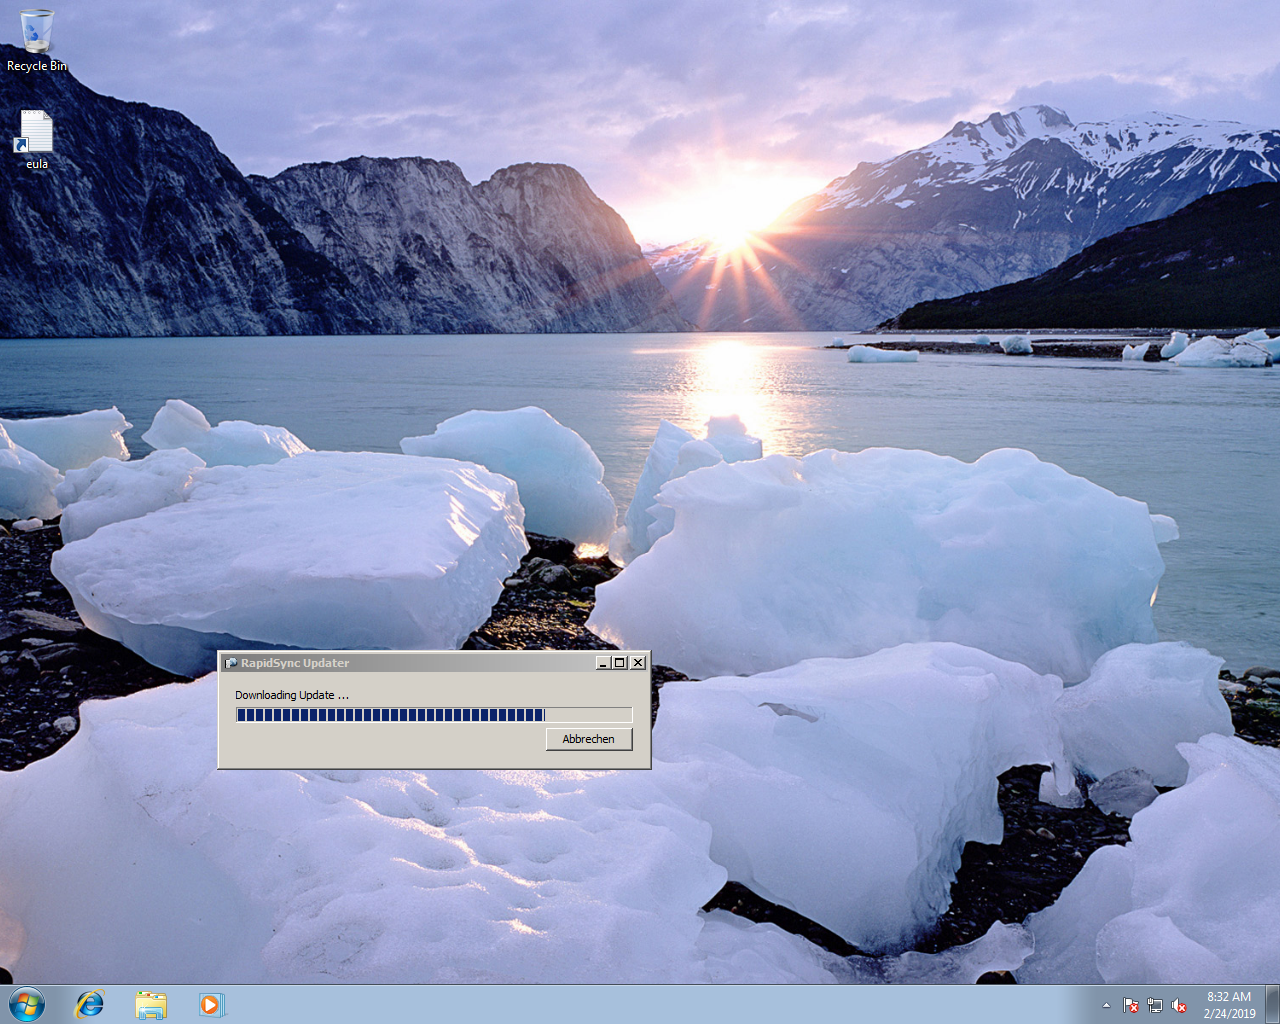
\includegraphics[width=0.4\textwidth]{fig/setup1-ex3}
				}\qquad
			\subfigure{
				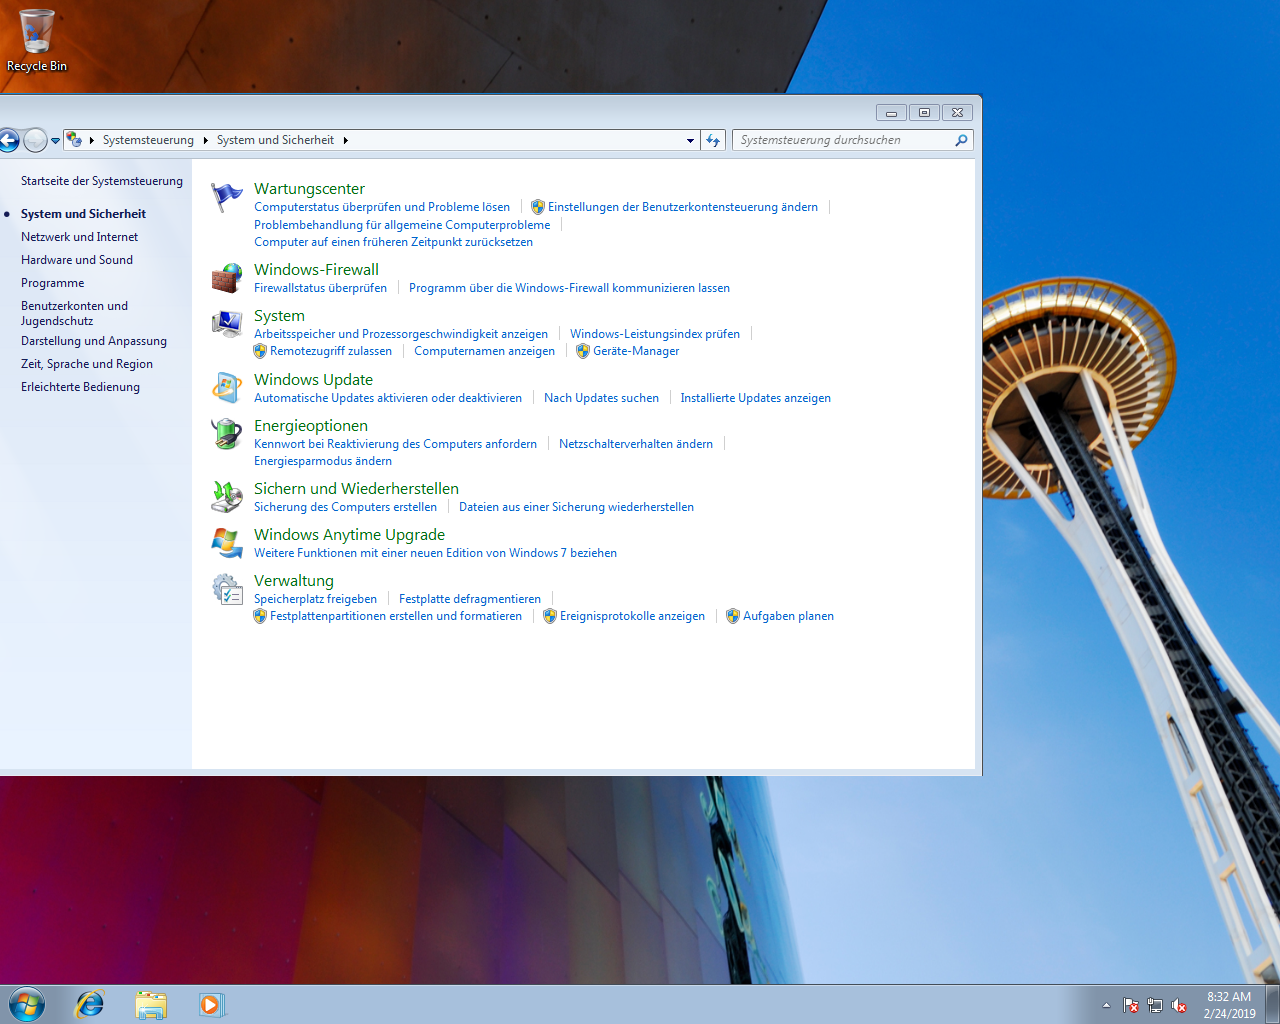
\includegraphics[width=0.4\textwidth]{fig/setup1-ex4}
				}\\
			\caption{Examples for screenshots of first evaluation setup.}
		\end{figure}
	\end{frame}
	
	\subsection{Results: Detection rate}
	\begin{frame}
		\frametitle{Results for the detection rate}
		% Confusion matrix
		\begin{figure}[h!]
			\subfigure{
				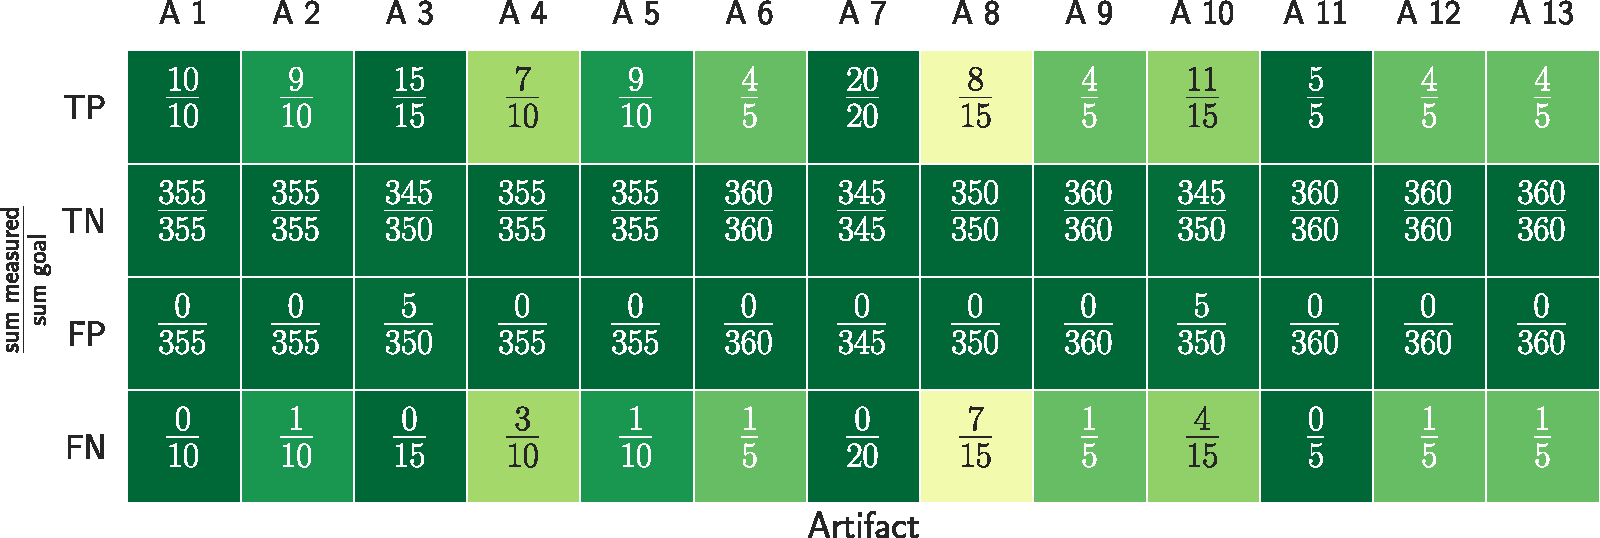
\includegraphics[width=0.9\textwidth]{fig/quality-confusion-matrix-p1}
				}\hfill\\
			\subfigure{
				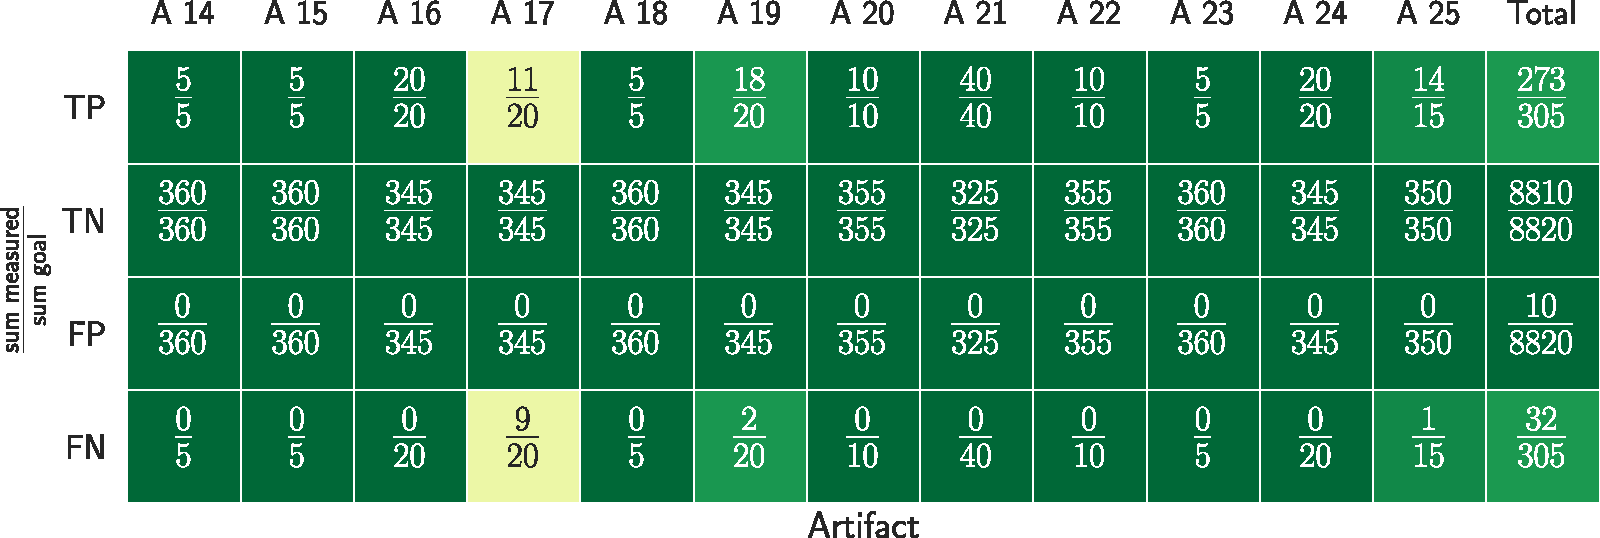
\includegraphics[width=0.9\textwidth]{fig/quality-confusion-matrix-p2}
				}\hfill\\
		\end{figure}
	\end{frame}
	
	\subsection{Results: Used resources}
	\begin{frame}
		\frametitle{Results of used resources}
		% Violin plot setup 1
		\begin{figure}[h!]
			\subfigure{
				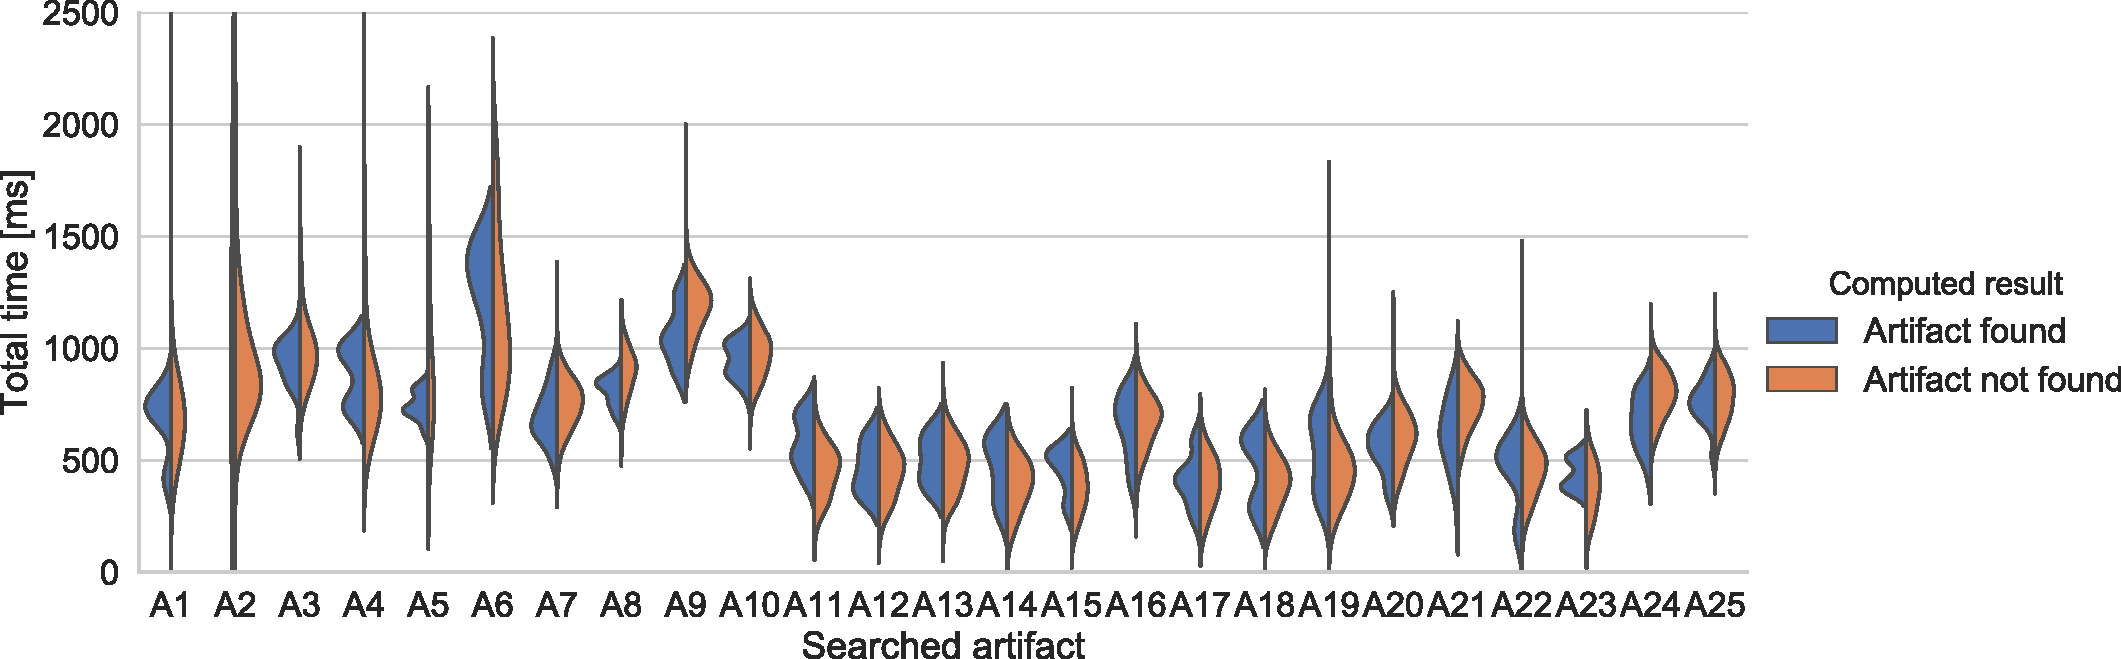
\includegraphics[width=0.9\textwidth]{fig/runtime-qualitative-02}
				}\hfill\\
			\subfigure{
				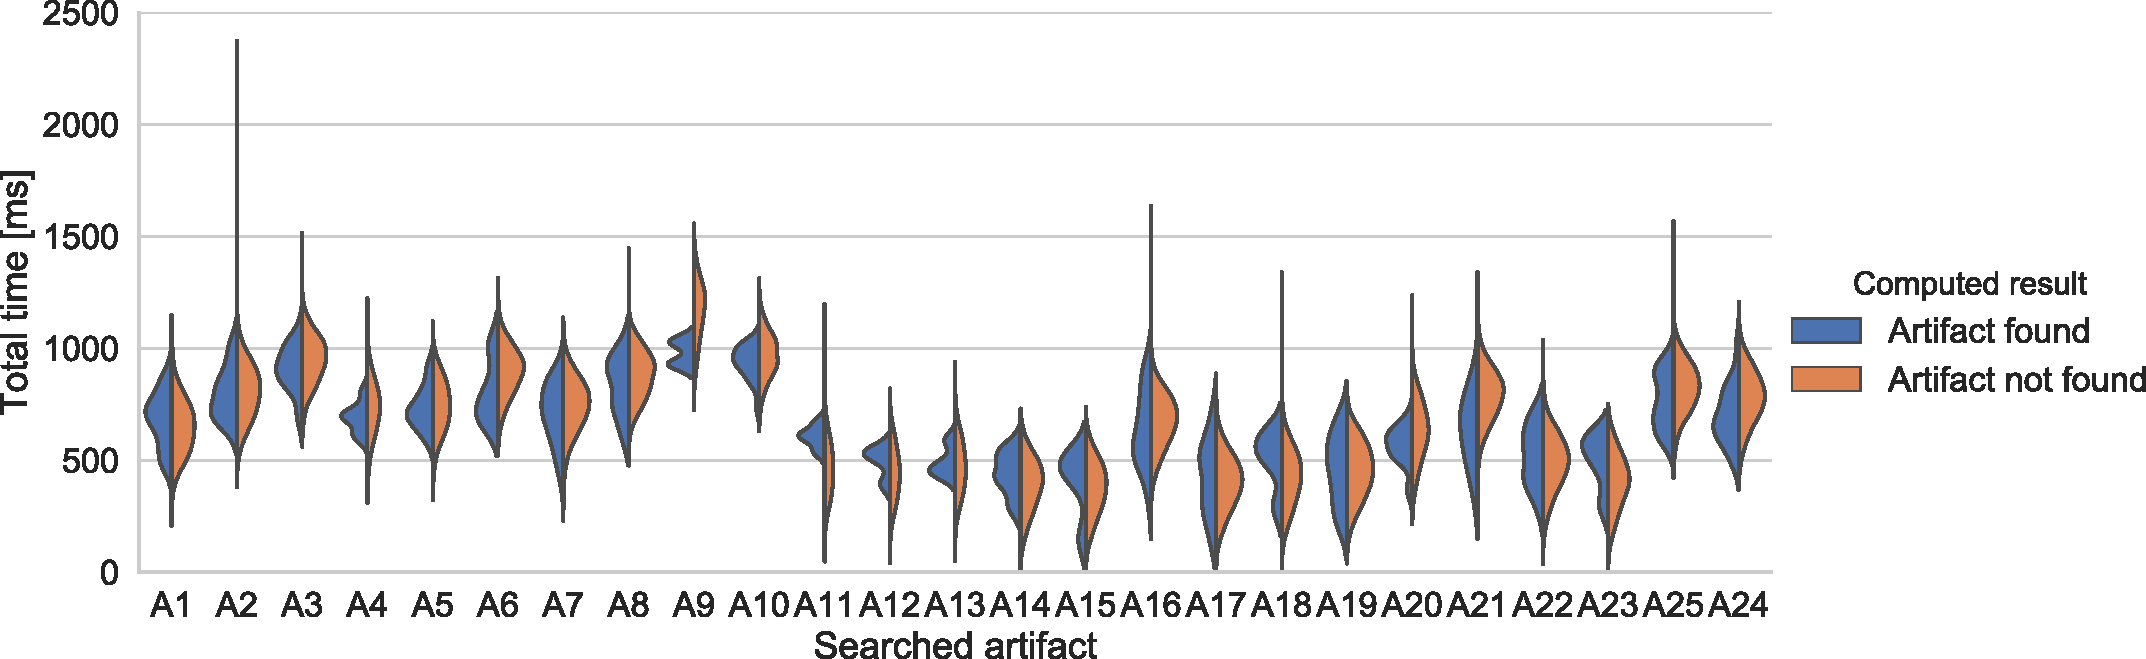
\includegraphics[width=0.9\textwidth]{fig/runtime-qualitative-03}
				}\hfill\\
		\end{figure}
	\end{frame}
	
	\begin{frame}
		% Setup 2
		% Structure setup 2
		\frametitle{Used Resources: Details? Factors?}
		First setup: Heterogeneity of artifact types; Too many confounding variables\\
		$\Rightarrow$ Second setup
		\pause
		\begin{itemize}
			\item Eight artifact types Q 0 to Q 7, two reference images $r_a$, $r_b$
			\item Two different screenshots: Artifact present ($s_{ap}$) and absent ($s_{aa}$)
			\item Each combination 1000 times
			\item 16000 executions of the VAD
		\end{itemize}
	\end{frame}
	
	\begin{frame}
		\begin{figure}[h!]
			\centering
			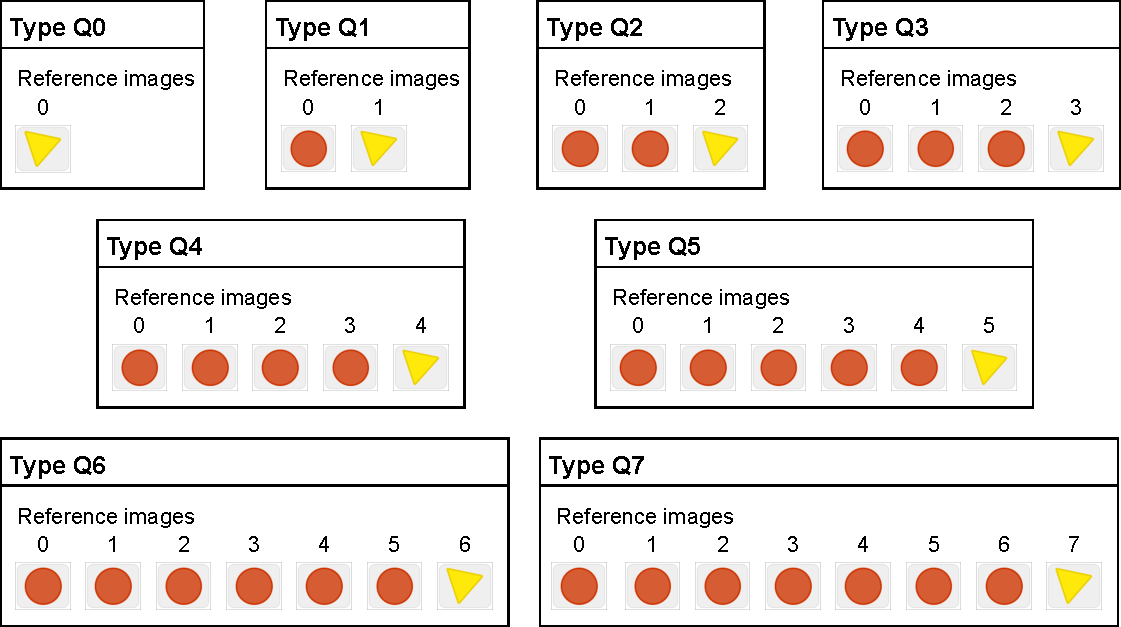
\includegraphics[width=0.8\textwidth]{fig/artifact_types_t2}
			\caption{Structure of the artifact types Q0 to Q7.}
		\end{figure}
	\end{frame}
	
	\begin{frame}
		\frametitle{Results for setup 2}
		\begin{figure}[h!]
			\centering
			\subfigure{
				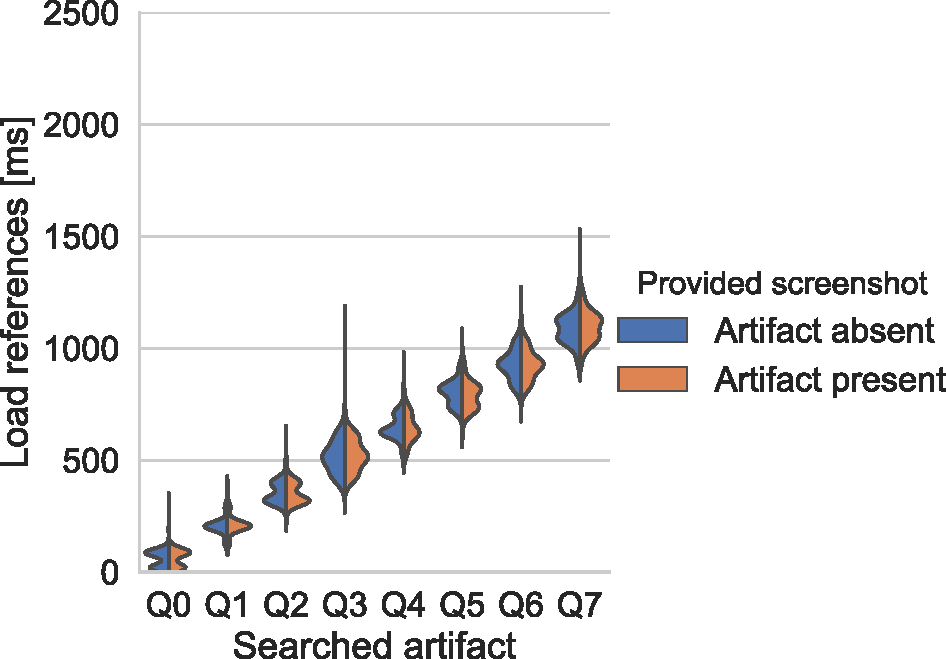
\includegraphics[width=0.4\textwidth]{fig/quantity-violin-load}
				}\qquad
			\subfigure{
				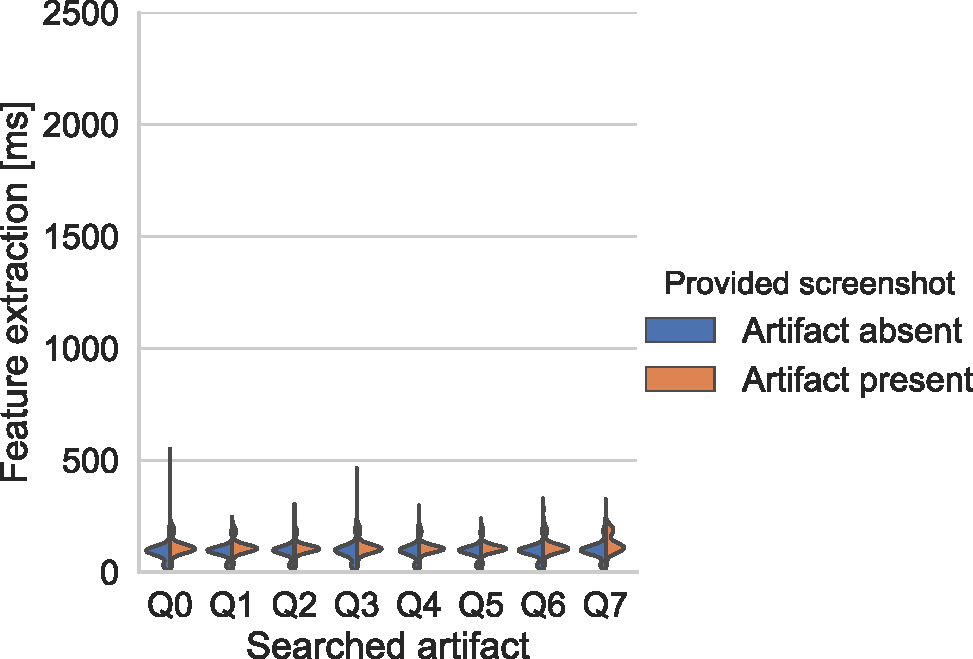
\includegraphics[width=0.4\textwidth]{fig/quantity-violin-feature_ext}
				}\\
			\subfigure{
				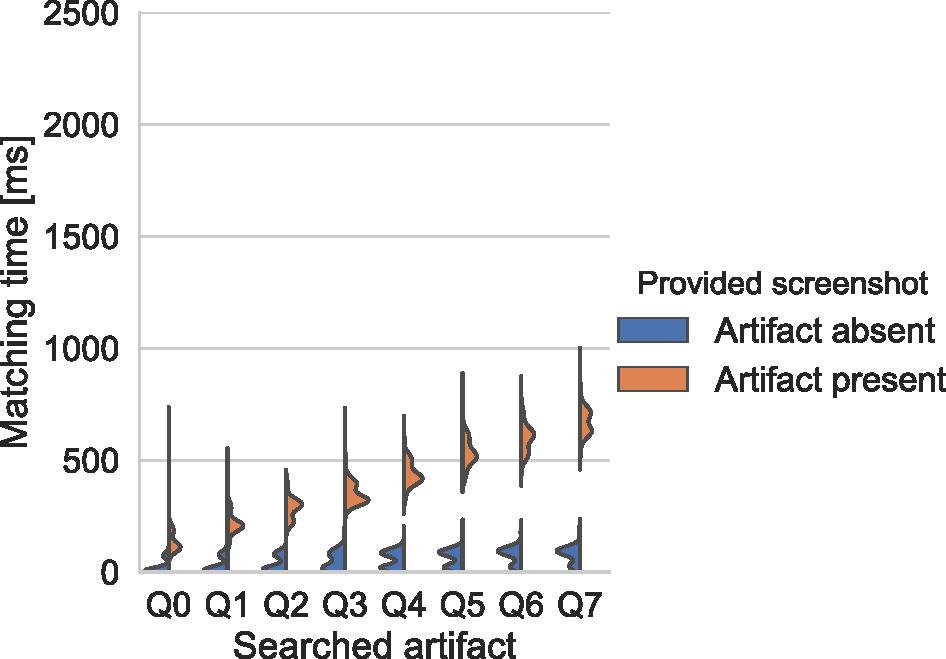
\includegraphics[width=0.4\textwidth]{fig/quantity-violin-matching}
				}\qquad
			\subfigure{
				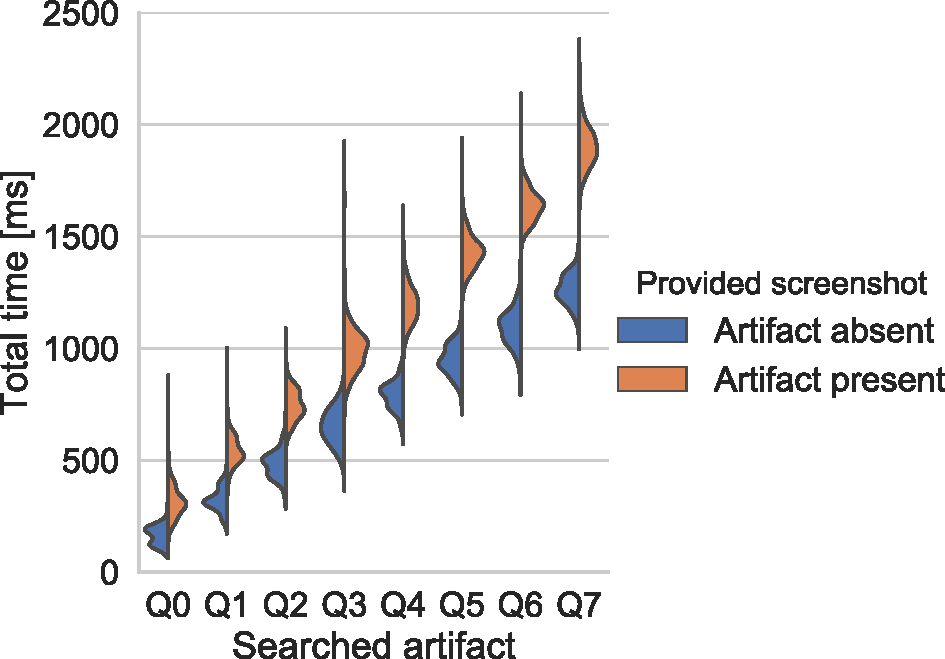
\includegraphics[width=0.4\textwidth]{fig/quantity-violin-total}
				}
			\caption{Execution time distributions for artifacts Q0 to Q7.}
		\end{figure}
	\end{frame}
	
	\begin{frame}
		\frametitle{Other resources}
		Measured at random times during all executions.
		\begin{itemize}
			\item $100\%$ CPU usage
			\item About 30 to 45MB RAM usage
		\end{itemize}
	\end{frame}
	
	\section{Conclusions}
	\begin{frame}
		\frametitle{Conclusions}
		% Yes yes, very success
		\begin{itemize}
			\item Successful implementation regarding detection
			\item Room for improvement for execution duration, but success for average
		\end{itemize}
		\pause
		Future work could include:
		\begin{itemize}
			\item Improvement of caching mechanism
		\end{itemize}
	\end{frame}
	
	\section{Discussion}
	\begin{frame}
		\frametitle{Thank you for listening!}
		Do you have any questions, remarks?
	\end{frame}
	
	\begin{frame}[shrink=40,fragile]
		\frametitle{Bibliography}
		\vspace*{1cm}~\\
		\bibliographystyle{alphadin}
		\bibliography{bibliography}
	\end{frame}
\end{document}